\documentclass[letterpaper,10pt]{article}
\usepackage[utf8x]{inputenc}
\usepackage[margin=1.25in]{geometry}
\usepackage{graphicx}
\usepackage{float}
\usepackage{amssymb}
\usepackage{amsmath}
\usepackage{enumerate}
\usepackage{amsthm}
\usepackage[parfill]{parskip}
\usepackage[round]{natbib}
\usepackage{multirow}

\newcommand{\al}{\ensuremath{\alpha}}
\newtheorem{thm}{Theorem}
\newcommand{\bs}{\ensuremath{\boldsymbol}}
\DeclareMathOperator*{\argmin}{arg\,min\;}
\DeclareMathOperator*{\diag}{diag}
\DeclareMathOperator*{\st}{subject\,to\;}

\title{Harmonic Analysis Final Paper \\ Incoherence and Structured Random Matrices}
\author{Keith Kelly, Yerlan Amanbek, and Sameer Tharakan}

\begin{document}
\maketitle
\section{Introduction}
%%%%%%%%%%%%%%%%%%%%%%%%%%%%%%%%%%%%%%
%% Frame
%%%%%%%%%%%%%%%%%%%%%%%%%%%%%%%%%%%%%%

\begin{frame}[t]
	\frametitle{Introduction}
	\framesubtitle{~~}  %% needed for proper positioning of the logo ...

	The Basis pursuit problem 
	\begin{equation}
		\min ||x||_{l_1} \quad \text{ subject to } \quad \Phi \Psi x=y
	\end{equation}

	\small
	Where $\Psi$ is an $n \times n$ orthogonal matrix corresponding to the basis in which our signal $z = \Psi x$ is $S$-sparse. $\Phi$ is our sensing matrix. 
	\\
	\normalfont
	\textbf{Toeplitz} and \textbf{Circulant} matrices have the forms, respectively,
	\\
	
	$$
	T = \begin{bmatrix}
		t_{1}    & t_{2}    & ...    & t_{n}   \\[0.3em]
		t_{n+1}  & t_{1}    & ...    & t_{n-1} \\[0.3em]
		\ddots   & \ddots   & \ddots &         \\[0.3em]
		t_{2n-1} & t_{2n-2} & ...    & t_{1}         
	\end{bmatrix}
	\qquad \text{and} \qquad
	C = \begin{bmatrix}
		t_{1}  & t_{2}  & ...    & t_{n}   \\[0.3em]
		t_{n}  & t_{1}  & ...    & t_{n-1} \\[0.3em]
		\ddots & \ddots & \ddots &         \\[0.3em]
		t_{2}  & t_{3}  & ...    & t_{1}        
	\end{bmatrix} 
	$$
\end{frame}
%%%%%%%%%%%%%%%%%%%%%%%%%%%%%%%%%%%%%
%% Frame
%%%%%%%%%%%%%%%%%%%%%%%%%%%%%%%%%%%%%%
\begin{frame}[t]
	\frametitle{Structured random matrices}
	\framesubtitle{~~}  %% needed for proper positioning of the logo ...
	Any Circulant matrix can be diagonalized by a Fourier transform, i.e. obeying
	$$ C=\frac{1}{\sqrt{n}} F^* \Sigma F $$ with $F$ as the discrete Fourier matrix
	$F_{t,w}=e^{-i\; 2\pi(t-1)(w-1)/n}, \qquad 1 \le t,w \le n$
	$$
	\Sigma = \begin{bmatrix}
		\sigma_{1} & 0 & ...& 0           \\[0.3em]
		0 & \sigma_{2} & ... & 0 \\[0.3em]
		\ddots &\ddots & \ddots &      \\[0.3em]
		0 & 0 & ... & \sigma_{n}        
	\end{bmatrix} $$
	a diagonal matrix whose entries are unit magnitude complex numbers with random phases.
\end{frame}


%%%%%%%%%%%%%%%%%%%%%%%%%%%%%%%%%%%%%
%% Frame
%%%%%%%%%%%%%%%%%%%%%%%%%%%%%%%%%%%%%%
\begin{frame}[t]
	\frametitle{Structured random matrices}
	\framesubtitle{~~}  %% needed for proper positioning of the logo ...
	We generate $\sigma_{w}$ as follows:
	\\[1em]

	$w=1\qquad \qquad \qquad : \; \sigma_{1} \sim \pm$ 1 with equal probability,
	\\[1em]
	$2 \le w < n/2+1 \; \; : \; \sigma_{w}=e^{i\theta w}, where \; {\theta}_{w} \sim Uniform(0,2\pi) $
	\\[1em]
	$w=n/2+1 \qquad \; \; \, : \; \sigma_{n/2+1} \sim \pm 1 $ with equal probability 
	\\[1em]

	$n/2+2 \le w \le n \; \; : \; \sigma_{w}=\sigma^{*}_{n-w+2}$, conjugate of  $\sigma_{n-w+2}$.
	
	$$
	$$
	Generating the diagonal in this way ensures the resulting circulant matrix is real-valued due 
	to conjugate symmetry.
\end{frame}

%%%%%%%%%%%%%%%%%%%%%%%%%%%%%%%%%%%%%%
%% Frame
%%%%%%%%%%%%%%%%%%%%%%%%%%
%%%%%%%%%%%%
\begin{frame}[t]
	\frametitle{Structured random matrices}
	\framesubtitle{~~}  %% needed for proper positioning of the logo ...
	$$
	T_{n} = \left[ \: 
		\begin{array}{*{4}{c}}
			\cline{1-4}
			\multicolumn{1}{|c}{t_{1}} & t_{2} & ...& \multicolumn{1}{c|}{t_{n}}           \\[0.3em]
			\cline{1-4}
			t_{n+1} & t_{1} & ... & t_{n-1} \\[0.3em]
			\ddots &\ddots & \ddots &    \\[0.3em]
			t_{2n-1} & t_{2n-2} & ... & t_{1}      \\[0.3em]    
		\end{array}
	\right]
	=
	\left[ \:
		\begin{array}{*{4}{c}}
			t_{1} & t_{2} & ...& t_{n}        \\[0.3em]
			\cline{1-1}
			\multicolumn{1}{|c|}{t_{n+1}} & t_{1} & ... & t_{n-1} \\[0.3em]
			\multicolumn{1}{|c|}{\ddots} & \ddots & \ddots &    \\[0.3em]
			\multicolumn{1}{|c|}{t_{2n-1}} & t_{2n-2} & ... & t_{1}          \\[0.3em]
			\cline{1-1}
		\end{array}
	\right]
	$$
	\\
	$$
	C_{2n} =\begin{bmatrix}
		t_{1}   & t_{2} & ...    & t_{n}  & 0   & t_{2n-1} & ... &  t_{n+1}   \\[0.3em]
		t_{n+1} & t_{1} & ...    & t_{n-1}& ... & 0  & ... &          \\[0.3em]
		\ddots  &       & \ddots &        & \ddots & & &\ddots    \\[0.3em]
		\cdots  &       & \cdots &       & \cdots & & & \cdots
	\end{bmatrix}
	=
	\begin{bmatrix}
		T_{n} & B_{n}            \\[0.3em]
		B_{n} & T_{n}   
	\end{bmatrix}
	$$

\end{frame}

%%%%%%%%%%%%%%%%%%%%%%%%%%%%%%%%%%%%%
%% Frame
%%%%%%%%%%%%%%%%%%%%%%%%%%%%%%%%%%%%%%
\begin{frame}[t]
	\frametitle{Structured random matrices}
	\framesubtitle{~~}  %% needed for proper positioning of the logo ...
	\textbf{Hadamard} matrix is a square matrix whose entries are either $+1$ or $-1$ and whose rows are mutually orthogonal.
	\begin{figure}[h]
		\centering
		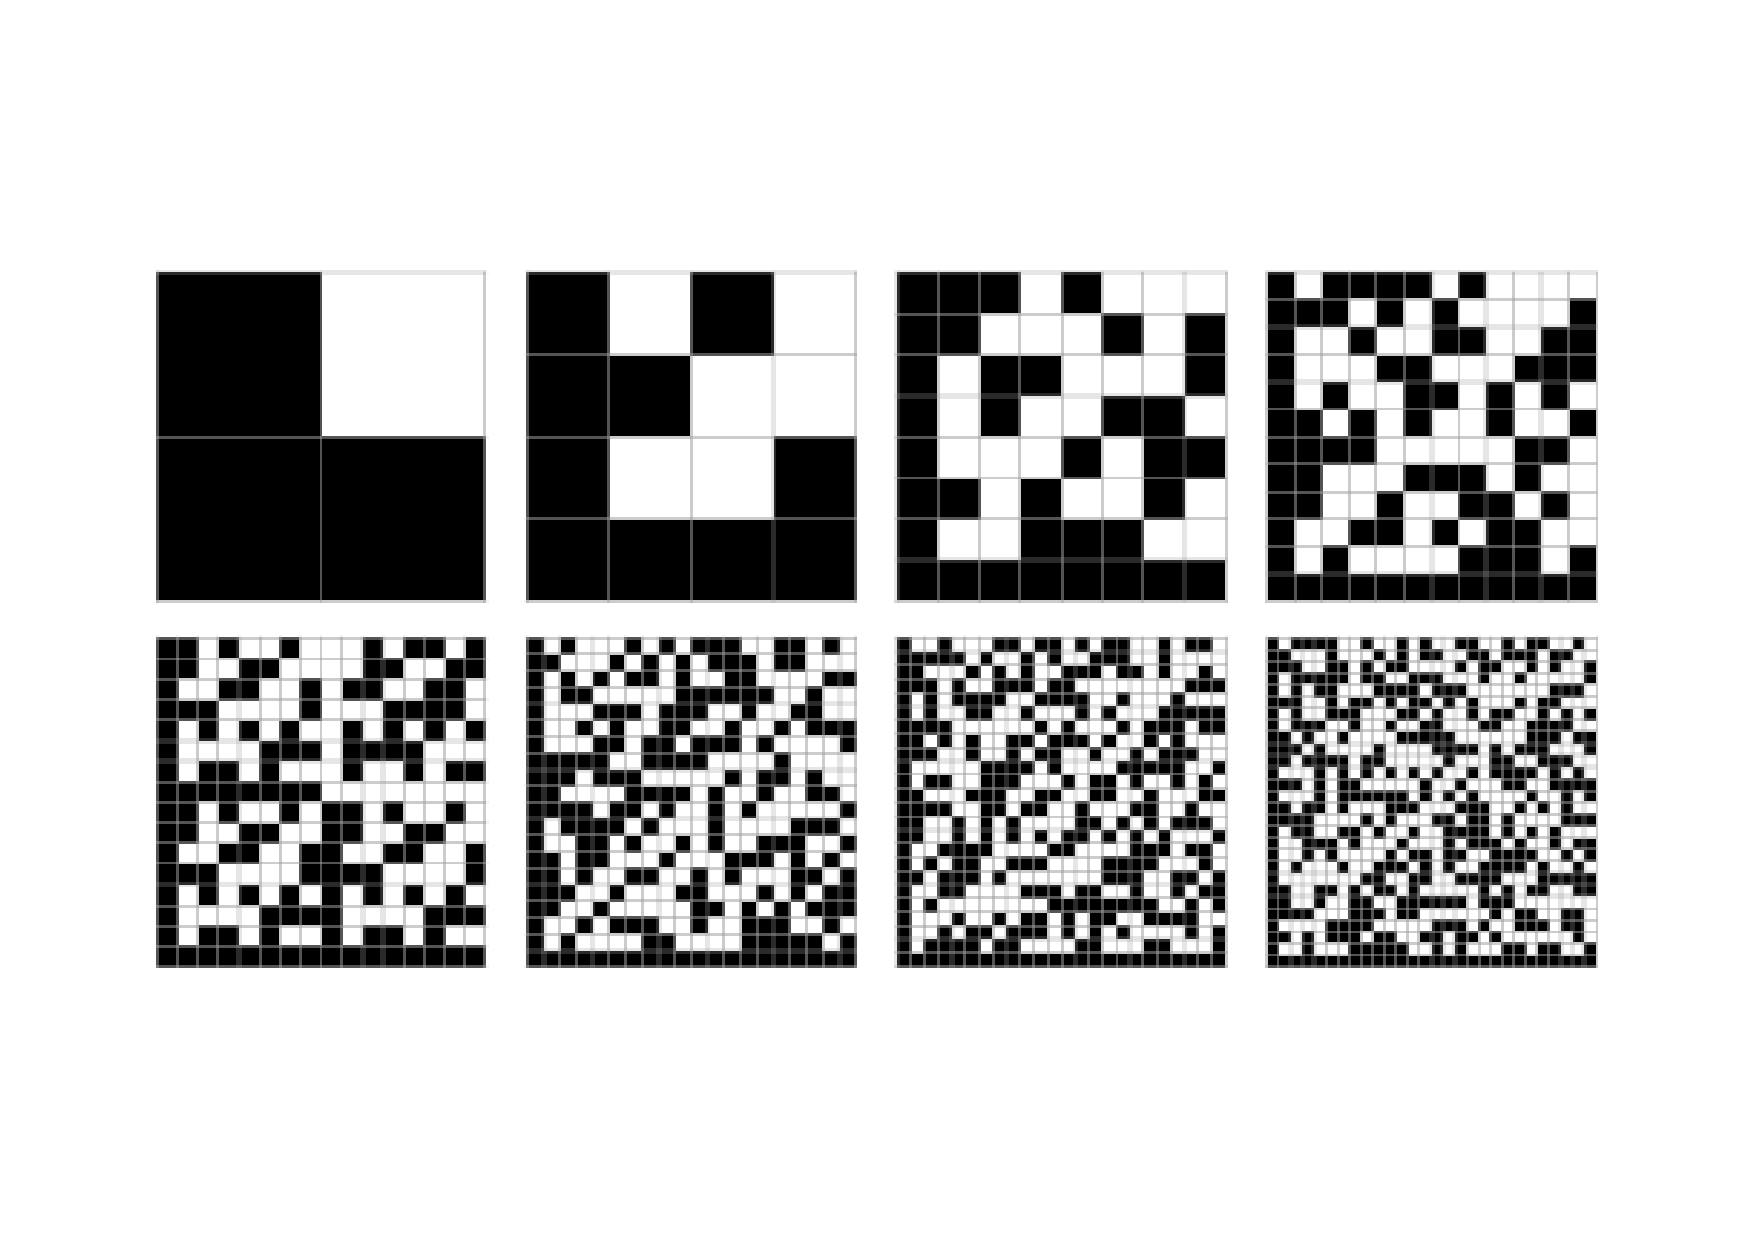
\includegraphics[width=0.7\linewidth]{HadamardMatrices_800}
		\caption{}
		\label{fig:HadamardMatrices_800}
	\end{figure}

\end{frame}
%%%%%%%%%%%%%%%%%%%%%%%%%%%%%%%%%%%%%%
%% Frame
%%%%%%%%%%%%%%%%%%%%%%%%%%%%%%%%%%%%%%
\begin{frame}[t]
	\frametitle{Structured random matrices}
	\framesubtitle{~~}  %% needed for proper positioning of the logo ...
	An equivalent definition of the Hadamard matrices is given by 
	$$ H_{n} H_{n}^T = n  I_{n} $$
	where $I_{n}$ is the $n \times n$ identity matrix.
	$$
	H_{1} = \begin{bmatrix}
		1
	\end{bmatrix}
	\qquad
	H_{2} = \begin{bmatrix}
		1 & 1           \\[0.3em]
		1& -1
	\end{bmatrix}	
	\qquad
	H_{4} = \begin{bmatrix}
		H_{2} & H_{2}           \\[0.3em]
		H_{2}& -H_{2}
	\end{bmatrix}	
	$$
	$$
	\centering
	\qquad
	H_{2^{n}} = \begin{bmatrix}
		H_{2^{n-1}} & H_{2^{n-1}}           \\[0.3em]
		H_{2^{n-1}}& -H_{2^{n-1}}            
	\end{bmatrix}	
	$$
\end{frame}



\subsection{Relation to Previous Work}
\paragraph{Parallel SVM}
Parallel SVM algorithms can broadly be classified into explicit and implicit approaches. Explicit approaches identify  independent components of the problem and use parallel frameworks such as OpenMP, MPI, CUDA/OpenCL or MapReduce to directly encode this parallelism. Implicit approaches represent the calculations required for the SVM problem via matrix operations for which highly optimized parallel libraries exist. These approaches have their own advantages and disadvantages some of which we will discuss below. A detailed comparison and empirical analysis of popular explicit and implicit approaches on CPUs and GPUs is presented in \cite{tyree2014parallel}.

Explicit approaches require code for the problem to be written by hand. This usually involves significant engineering effort and requires fine-tuning of the tradeoffs between parallel work and framework overhead. The underlying algorithm for explicit approaches may be based on Platt's SMO algorithm~\citep{platt1999fast}, interior point approaches or gradient projection approaches. However, \cite{brugger2006parallel} and \cite{tyree2014parallel} note that competitive approaches in this vein are usually based on SMO and other similar dual decomposition procedures. SMO considers two variables and performs a block coordinate-descent w.r.t. these two variables. It is also possible to consider larger groups of variables for each iteration and various approaches have been proposed to split the SVM problem into subproblems which can be solved in parallel~\citep{cao2006parallel, collobert2002parallel, graf2004parallel, zhang2005parallel}. Of special interest to this paper is DC-SVM~\citep{hsieh2013divide}, which divides the data into subproblems based on a hierarchical clustering. \cite{hazan2008parallel} consider a decomposition based on Fenchel duality.  PSVM~\citep{zhu2008parallelizing} proposes a distributed algorithm for SVMs. \cite{zhao2011parallel} propose a parallel SVM algorithm in the MapReduce framework. GTSVM~\citep{cotter2011gpu} harness the specific capabilities of GPUs. 

In addition to the individual iterations, kernel computations make up a significant portion of the overall computation time and can also be parallelized. The multicore version of LibSVM~\citep{chang2011libsvm} includes only this parallelization with OpenMP and this results in a significant significant speedup.

Implicit parallelization approaches formulate the SVM problem as matrix-vector multiplications and use optimized parallel linear algebra libraries for the parallelism. \cite{sha2002multiplicative} propose a multiplicative update rule to solve SVMs, however directly implementing this method requires the (dense) kernel matrix to be stored explicity and is thus memory-intensive. \cite{chapelle2007training} present a multiplicative algorithm for the squared hinge loss via dense matrix operations. \cite{keerthi2006building} reduce the complexity of this approach by using a sparse basis set for the dual variables so that only part of the kernel matrix needs to be computed. This approach is known as Sparse Primal SVM (SP-SVM) and lends itself to easy implicit parallelization. \cite{tyree2014parallel} show that this method is very efficient for medium-scale datasets.

Our algorithm is also an explicit algorithm based on a no-bias version of the SVM problem which reduces to coordinate descent similar to that in \cite{hsieh2013divide}, and we use Galois (described below) as a parallel framework.

\paragraph{Galois}
Galois is a parallel framework based on the operator-schedule paradigm introduced in \cite{pingali2011tao}. A parallel Galois program is expressed via a parallel operator which operates on a node in a graph, and a schedule specifying the order in which nodes should be operated on. The schedule can be modified by the program as it executes and thus allows for \emph{data-dependent parallelism}. The operator is only allowed to access information for the node it is operating on and its neighbours, thus serializability can be maintained by allowing only non-adjacent nodes to be processed simultaneously.

For no-bias SVM solved with dual coordinate descent as in the present work, each data point corresponds to a node in the graph and edges in the graph indicate whether those nodes are independent according to Theorem~\ref{thm:serializabilty}. For coordinate descent, the choice of schedule does not affect convergence, but it is expected to affect the rate of convergence.

\section{Experiments}
We ran two types of tests to validate that preexisiting models worked and were
comparable to our proposed sensing matrices that combined the two types of
models. In one, we simulate compressed sensing by creating sensing operators,
measuring an image and then solving a TV-minimization problem to attempt to
recover the image. We then compare the recovered image to the original to
determine the relative error. Concretely, we compute the relative error
$\varepsilon$ as

\begin{equation}
  \frac{||x^{\#} - x||_2}{||x||_2} = \varepsilon
\end{equation}

and compare this error for each of the possible methods considered. In the other
test, we were only interested in the time to compute the solution $x^{\#}$ for
the various types of methods. In particular, we wanted to show that the
structured random matrices are much more efficient than using a completely
random matrix with Gaussian i.i.d. entries. In neither case is there any
appreciable amount of noise added to the measurements and in general we will
not show the reconstructed images since for our experiments the construction
quality was good enough across the board that differences between the images
were not meaningfully discernable. 

In the first experiment we tested our method on a $128 \times 128$ modified
Shepp-Logan phantom test image and used $128^2/3$ measurement samples for our
data to reconstruct the image. Figure \ref{fig:shepplogan} shows an example of
this image and its reconstruction.


\begin{figure}[h!]
  \centering
  \caption{Modified Shepp-Logan phantom reconstructed using a circulant matrix with RPMS restriction.}
  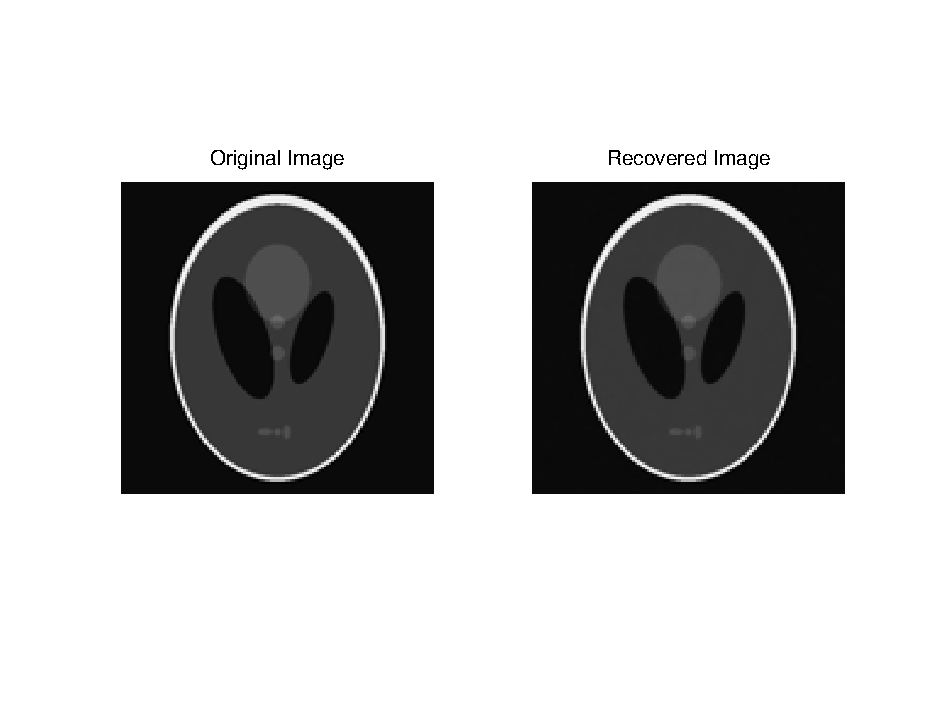
\includegraphics[width=0.6\textwidth, trim= 0 40 0 40, clip=true]{figs/rpms.pdf}
  \label{fig:shepplogan}
\end{figure}


\begin{table}[h] 
  \begin{tabular}{lll|lllll} 
    \textbf{Matrix Type}       & \textbf{Input Randomizer} & \textbf{Output Randomizer} & \textbf{Error} & \textbf{Time}  & \\ \hline
    \multirow{2}{*}{Circulant} & \multirow{2}{*}{N/A}      & Sub                        & 0.0156         & 4.97s          & \\
                               &                           & RPMS                       & 0.0159         & 7.80s          & \\ \hline
    \multirow{2}{*}{Toeplitz}  & \multirow{2}{*}{N/A}      & Sub                        & 0.0193         & 25.9s          & \\ 
                               &                           & RPMS                       & 0.0170         & 16.9s          & \\ \hline
    \multirow{4}{*}{Fourier}   & \multirow{2}{*}{Local}    & Sub                        & 0.0183         & 7.89s          & \\ 
                               &                           & RPMS                       & 0.0517         & 14.0s          & \\             
                               &  \multirow{2}{*}{Global}  & Sub                        & 0.0166         & 4.98s          & \\ 
                               &                           & RPMS                       & 0.0529         & 14.1s          & \\ \hline
    \multirow{4}{*}{Hadamard}  & \multirow{2}{*}{Local}    & Sub                        & 0.0167         & 552s           & \\
                               &                           & RPMS                       & 0.0153         & 752s           & \\
                               & \multirow{2}{*}{Global}   & Sub                        & 0.0157         & 544s           & \\
                               &                           & RPMS                       & 0.0137         & 782s           & \\
  \end{tabular} 
\caption{Table of reconstruction error $\varepsilon$ and timing results for all it the structured sensing matrices described previously.}
\label{tab:errors}
\end{table}

Table \ref{tab:errors} summarizes the results of our first experiment comparing
the solution accuracy of the various sensing matrices and input and output
randomizers. We do not use an input randomizer with circulant or Toeplitz
matrices since we could not converge to a solution using those methods. We see
that the reconstruction errors for almost all of the methods are comparable.
However, in the case of a Fourier transform sensing matrix with RPMS
subsampling operator does not work well. In addation to not achieving a
solution as good as the othertested methods, it showed poor convergence
compared to the simpler subsampling methods in the sense that it took longer to
converge. We are not convinced that the RPMS method is working in that case,
but that it is functioning correctly for circulant, Toeplitz and Hadamard
sensing matrices (where we are unaware of it having ever been used before). 

\begin{table}[h]
  \begin{tabular}{l|lllllll} 
    \textbf{Matrix Type} & Gaussian & Circulant & Toeplitz & Fourier & Hadamard \\ \hline
    \textbf{Time}        & 12.2s    & 1.65s     & 4.24s    & 1.50s   & 102s*    \\ 
  \end{tabular}
  \label{tab:times}
  \caption{ In this table we see how the time to compute the
    solution for a smaller problem using the random structured sensing
    operators compares with the time to compute the solution using a completely
    random matrix with Gaussian i.i.d. entries. *The fast Walsh-Hadamard
    transform in \textsc{Matlab} is written in \textsc{Matlab} and is slow.}
  \end{table}

In the second experiment we used the same test image scaled by a factor of a
half because the testing machine that we were using could not handle solving
the slightly larger (yet still small) problem using the completely random
matrix in  a reasonable amount of time. This was due to not only the complexity
of computing matrix-vector products with the random matrix, but also due to
memory restructions.

Table \ref{tab:times} summarizes the results of the second experiment. We see
that the the structured random matrices are able to compute the solution much
more quickly than the completely random matrix, with the exception of the
operator using the fast Walsh-Hadamard transform, which suffers from a slow
implementation in \textsc{Matlab}. However, the transform has the same
complexity as the FFT and so we expect that if the two were implemented
similarly, that thet should exhibit similar performance.  The Toeplitz based
sensing matrix is a little slower than the others using a fast transform, but
this is expected since performing a fast Toeplitz matrix-vector multiplication
requires using an FFT on a vector that is twice the size of the one you wish to
multiply. 

Overall the tests indicate the importance of the fast transforms for large
problems and the possibility of using the RPMS restriction operator with
sensing matrices other than circulant as originally suggested in
\cite{romberg2009}.


\section{Future Work}
There are various parts to this project which we were not yet able to address:
\begin{itemize}
	\item We would like to see empirically how sparsity affects each of the methods we 
		have looked at to compare with the theory. In 
		\cite{wotao}, they had some results, but not for most of the matrices we 
		compared here. 
	\item We did most minimizations in the $TV$ norm, but we would like to see an 
		implementation of an ADMM (alternating direction method of multipliers) on an
		objective function containing both the $L_1$ and the $TV$ norms. \cite{wotao}
		implemented this, but not with the randomizations discussed here. 
\end{itemize}


\bibliographystyle{plainnat}
\nocite{*}
\bibliography{references}

\end{document}
